\documentclass[../main.tex]{subfiles}

\begin{document}

\subsubsection*{Methodology}
    In this section we move the laser medium along the orthogonal axis of the resonator and measure the output power $P_{HeNe}$ of the HeNe laser as a function of its deplacement $\Delta L$. We used a stepsize of $\delta L = (2.5\pm 0.1)\;\si{\cm}$ and a linear displacement in $10$ steps following $s(n) = \delta L\cdot n + L_0$ with $L_0 = (36.0\pm 0.1)\;\si{\cm}$ being the initial position of the laser medium. After every displacement we optimized again for laser output power by adjusting the $8$ screws of the setup. 
\subsubsection*{Data analysis}
    Because of the very small uncertaintys we neglected them while plotting the data points. Furhermore we measured a displacement $P_{fl}$ every time we moved the laser medium, which we subtracted from the measured output power. Figure \ref{fig:output_power_over_displacement} shows the adjusted output power of the HeNe laser as a function of the displacement of the active medium.

    \begin{figure}[H]
        \centering
        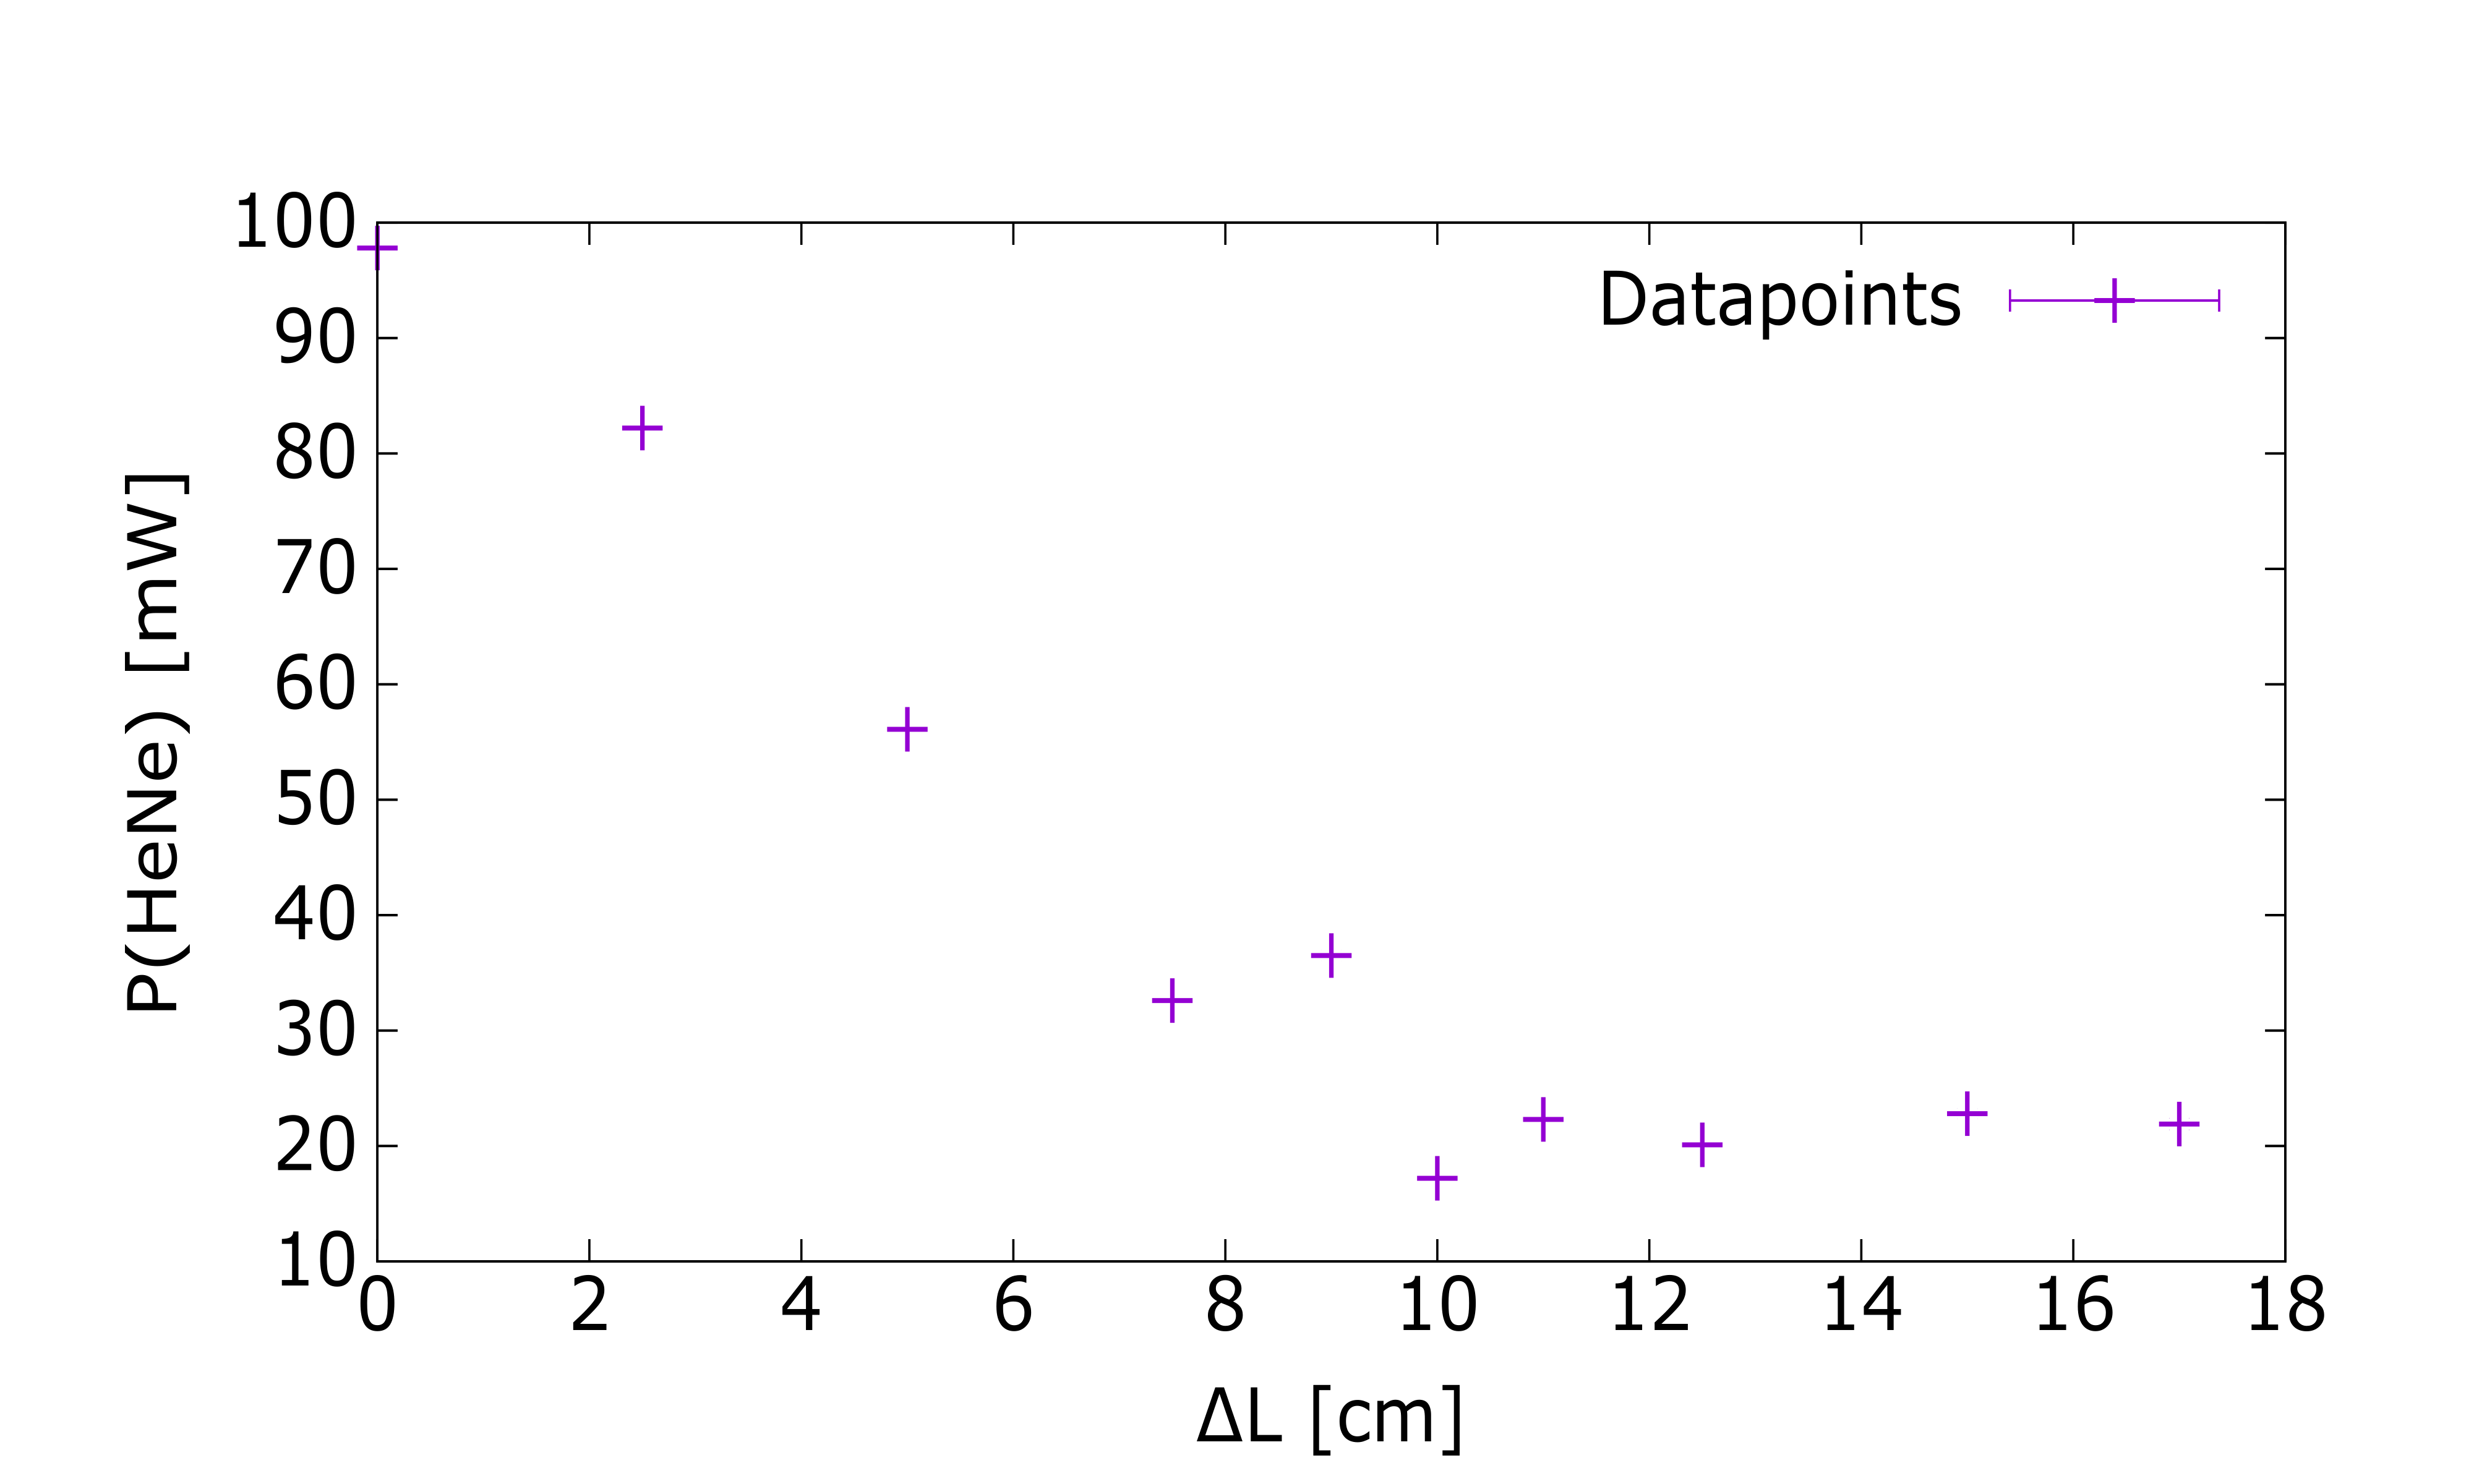
\includegraphics[width=0.8\textwidth]{Bilddateien/3/P(HeNe)overDx-adjusted.png}
        \caption{The output power of the HeNe laser as a function of the displacement of the active medium, starting at $L_0:=\SI{35.5(1)}{\cm}$ on the given scale.}
        \label{fig:output_power_over_displacement}
    \end{figure}

    Looking at figure \ref{fig:output_power_over_displacement} we can see a linear dependency in the beginning inteval $[2,10]$. The fast decline in lasing power could be explained by the defocused reflextion beams inside the resonator, which was curved at one end and linear at the other, from which we deplaced the medium in the experiment. Therefore the effective beam cross-section decreases and the possibility of stimulated emission decreases with it.

\end{document}